\documentclass[12pt, twoside]{article}
\linespread{1.15}
\usepackage[utf8]{inputenc}  % Ensure this is loaded before biblatex
\usepackage[sorting=none]{biblatex}  % Load the biblatex package
\usepackage{pdfpages}
\addbibresource{./../Quellen/sources.bib}  % Add your .bib file


%%%%%%%%%%%%%%%%%%%%%%%%%%%%% Using Packages %%%%%%%%%%%%%%%%%%%%%%%%%%%%%%%%%%
\usepackage[a4paper, margin=2cm, top=5mm, includehead, headheight=2cm]{geometry}
\usepackage{graphicx}
\usepackage{amssymb}
\usepackage{amsmath}
\usepackage{amsthm}
\usepackage{empheq}
\usepackage{mdframed}
\usepackage{booktabs}
\usepackage{lipsum}
\usepackage{graphicx}
\usepackage{color}
\usepackage{psfrag}
\usepackage{pgfplots}
\usepackage{bm}
\usepackage{float}
\usepackage{wrapfig}
\usepackage{enumitem}
\usepackage[export]{adjustbox} % for valign option
\usepackage{caption}
\usepackage{subcaption}
\usepackage{hyperref}
\usepackage{array}
\usepackage{tabularx}
\newcolumntype{P}[1]{>{\centering\arraybackslash}p{#1}}
\usepackage{tocloft}
\usepackage[section]{placeins}
\usepackage[nottoc,numbib]{tocbibind}
\usepackage{ragged2e}
\usepackage{pdfpages}
\usepackage[autostyle=true,german=quotes]{csquotes}
\usepackage{siunitx}
\sisetup{locale = DE} 
\usepackage{emptypage}
\usepackage{fancyhdr}
\usepackage{booktabs}
\usepackage{tabularx}
\usepackage{array}
\usepackage{longtable}
\usepackage{multirow}
\usepackage{pdfpages}

\usepackage{helvet}

\renewcommand{\familydefault}{\sfdefault}

\renewcommand{\footrulewidth}{0.4pt}%
\renewcommand{\headrulewidth}{0.4pt}%

\renewcommand{\headruleskip}{3mm}
\renewcommand{\footruleskip}{4mm}

\usepackage[main = ngerman, english]{babel}
\usepackage[ddmmyyyy]{datetime}

\newcommand{\todayD}{\the\day.\the\month.\the\year}   

\graphicspath{{../Bilder/}}

\setlength\parindent{0pt}
\counterwithin{figure}{section}
\counterwithin{table}{section}


\clubpenalty=10000
\widowpenalty=10000
\displaywidowpenalty=10000

\let\oldsection\paragraph
\renewcommand{\paragraph}[1]{\needspace{3\baselineskip}\oldsection{#1}}
%%%%%%%%%%%%%%%%%%%%%%%%%%%%%%%%%%%%%%%%%%%%%%%%%%%%%%%%%%%%%%%%%%%%%%%%%%%%%%%
\newcommand{\uni}[1]{\ensuremath{\, \mathrm{#1}}}
\DeclareSIUnit{\Umdrehung}{U}
% Other Settings
\usepackage[dvipsnames]{xcolor}

%\pagecolor[rgb]{0,0,0} %black

%\color[rgb]{0.5,0.5,0.5} %grey

%uncomment to make the links not display the red border
\hypersetup{
    colorlinks,
    citecolor=black,
    filecolor=black,
    linkcolor=black,
    urlcolor=black
}

\sisetup{
detect-all
}


%% codestuff
\usepackage{listings, listings-rust}
\renewcommand{\lstlistingname}{Code-Snippet}

\renewcommand{\lstlistlistingname}{Code-Snippets}
\setlength{\parindent}{8pt}
\usepackage{indentfirst}
\definecolor{codegreen}{rgb}{0,0.6,0}
\definecolor{codegray}{rgb}{0.5,0.5,0.5}
\definecolor{codecomment}{rgb}{0.6,0.6,0.6}
\definecolor{backcolour}{rgb}{1,1,1}
\definecolor{lightgray}{rgb}{.9,.9,.9}
\definecolor{darkgray}{rgb}{.4,.4,.4}
\definecolor{codepurple}{rgb}{0.65, 0.12, 0.82}

\lstdefinelanguage{JavaScript}{
    backgroundcolor=\color{backcolour},   
    keywords={typeof, new, true, false, catch, function, return, null, catch, switch, var, if, in, while, do, else, case, break},
    keywordstyle=\color{NavyBlue},
    ndkeywords={class, export, boolean, throw, implements, import, this},
    ndkeywordstyle=\color{codegray},
    identifierstyle=\color{black},
    sensitive=false,
    comment=[l]{//},
    morecomment=[s]{/*}{*/},
    commentstyle=\color{codecomment},
    stringstyle=\color{codepurple}\ttfamily,
    morestring=[b]',
    morestring=[b]",
    xleftmargin=1cm,
    captionpos=b
}

\lstdefinestyle{mystyle}{
    basicstyle=\fontsize{10}{12},
    backgroundcolor=\color{backcolour},   
    commentstyle=\color{codecomment},
    keywordstyle=\color{NavyBlue},
    numberstyle=\tiny\color{codegray},
    stringstyle=\color{codepurple},
    basicstyle=\ttfamily\footnotesize\bfseries,
    breakatwhitespace=false,         
    breaklines=true,                 
    captionpos=t,                    
    keepspaces=true,                 
    numbers=left,
    numbersep=5pt,                  
    showspaces=false,                
    showstringspaces=false,
    showtabs=false,                  
    tabsize=2,
    xleftmargin=1cm,
    captionpos=b
}
% -- Setting up the custom style:
\lstset{style=mystyle}

%%%%%%%%%%%%%%%%%%%%%%%%%% Page Setting %%%%%%%%%%%%%%%%%%%%%%%%%%%%%%%%%%%%%%%
\geometry{a4paper}

\newcommand{\iu}{{i\mkern1mu}}
\newcommand*\mathinhead[2]{\texorpdfstring{$\boldsymbol{#1}$}{#2}}

\definecolor{mred}{rgb}{0.619, 0.2392, 0.3176}


%%%%%%%%%%%%%%%%%%%%%%%%%%%%%%% Title & Author %%%%%%%%%%%%%%%%%%%%%%%%%%%%%%%%
\title{AFSS - Automated Factory Storage System}
\author{Benedikt Simbürger \\
    \and Nikolaj Voglauer \\
    \and Vincent Sonvilla \\
    \and Elena Widmann
    }

%%%%%%%%%%%%%%%%%%%%%%%%%%%%%%%%%%%%%%%%%%%%%%%%%%%%%%%%%%%%%%%%%%%%%%%%%%%%%%%
\babelprovide[import]{ngerman}


\fancyhf{}

\fancyhf[EHL]{\includegraphics[width=0.2\textwidth]{HTL_Moessingerstraßen_Logo.png}}
\fancyhf[OHL]{\includegraphics[width=0.2\textwidth]{HTL_Moessingerstraßen_Logo.png}}

\fancyhf[EHC]{\begin{tabular}{cc}
    Simbürger & Sonvilla \\
    Voglauer & Widmann \\
\end{tabular}}

\fancyhf[OHC]{\begin{tabular}{cc}
    Simbürger & Sonvilla \\
    Voglauer & Widmann\\
\end{tabular}}


\fancyhf[EFL]{\todayD}
\fancyhf[EFR]{\thepage}
\fancyhf[EHR]{\color{mred} ELEKTROTECHNIK}


\fancyhf[OFR]{\todayD}
\fancyhf[OFL]{\thepage}
\fancyhf[OHR]{\color{mred} ELEKTROTECHNIK}

\fancyhf[EFC]{Automated-Factory-Storage-System}
\fancyhf[OFC]{Automated-Factory-Storage-System}

\raggedbottom

\begin{document}
\sloppy
\pagenumbering{gobble}

\setlength{\parindent}{0pt}

\begin{figure}[h]
    \vspace{-5mm}
    \includegraphics[width=0.5\textwidth]{HTL_Moessingerstraßen_Logo.png}
    \centering
\end{figure}

\begin{center}
    \Large \textbf{HÖHERE TECHNISCHE BUNDESLEHRANSTALT} \\
    \vspace{5mm}
    \Large{KLAGENFURT, MÖSSINGERSTRASSE}

\end{center}

\vspace{7mm}

\begin{center}
    \Large{ABTEILUNG ELEKTROTECHNIK}
\end{center}

\hrule

\vspace{10mm}

\begin{center}
    \Huge \textbf{DIPLOMARBEIT} \\
    \vspace{7mm}
    \huge{Titel der Diplomarbeit Deutsch}

    \vspace{7mm}
    \huge{Automated-Factory-Storage-System}

    \vspace{7mm}
    \Large{JAHRGANG 5AHET}

\end{center}

\vspace{15mm}

\begin{flushleft}
    \linespread{1}
    \bgroup
        \large
        \def\arraystretch{1.5}
        \begin{tabular}{p{5cm}l}
            eingereicht von & Benedikt Simbürger\\
            & Vincent Sonvilla\\
            & Nikolaj Voglauer\\
            & Elena Widmann\\
            Projektbetreuer & Dipl.-Ing. Christian Sallinger
        \end{tabular}
    \egroup
\end{flushleft}

\vspace{7mm}
\large
Diese Diplomarbeit entspricht den Standards gemäß dem Leitfaden zur Umsetzung der Reife- und Diplomprüfung des BMBWF in der letztgültigen Fassung.\par
\begin{flushright}
    Klagenfurt, am 04.04.2025
\end{flushright}

\newpage

\begin{figure}[h]
    \includegraphics[width=0.5\textwidth]{HTL_Moessingerstraßen_Logo.png}
    \centering
\end{figure}

\begin{center}
    \huge \textbf{EIDESSTATTLICHE ERKLÄRUNG}\\
    \vspace{7mm}
    \large
    \begin{tabular}{p{14cm}}
        Ich versichere an Eides statt, dass ich diese Diplomarbeit
        selbstständig verfasst und keine anderen als die angegebenen
        Quellen und Hilfsmittel verwendet habe. Alle Gedanken, die im
        Wortlaut oder in grundlegenden Inhalten aus unveröffentlichten
        Texten oder aus veröffentlichter Literatur übernommen, oder mit
        künstlicher Intelligenz generiert wurden, sind ordnungsgemäß
        gekennzeichnet, zitiert und mit genauer Quellenangabe
        versehen.
    \end{tabular}

    \vspace{10mm}
    Verfasser/Verfasserin\\
    \vspace{10mm}
    \begin{tabular}{P{67mm}cP{67mm}}
        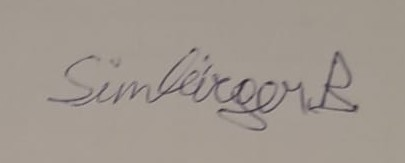
\includegraphics[width=60mm]{sign_simbuerger.jpg} & & 
\includegraphics[width=60mm]{sign_sonvilla.jpg} \\
        \cline{1-1}
        \cline{3-3}
        Benedikt Simbürger & & Vincent Sonvilla\\
    \end{tabular}
    

    
    \begin{tabular}{P{67mm}cP{67mm}}
        
\includegraphics[width=60mm]{sign_voglauer.png} & & 
\includegraphics[width=60mm]{sign_widmann.jpg} \\
        \cline{1-1}
        \cline{3-3}
        Nikolaj Voglauer & & Elena Widmann\\
    \end{tabular}

    \vspace*{\fill}
    \raggedleft Klagenfurt, am 04.04.2025

\end{center}

\newpage

\pagestyle{fancy}
\pagenumbering{arabic}
\normalsize

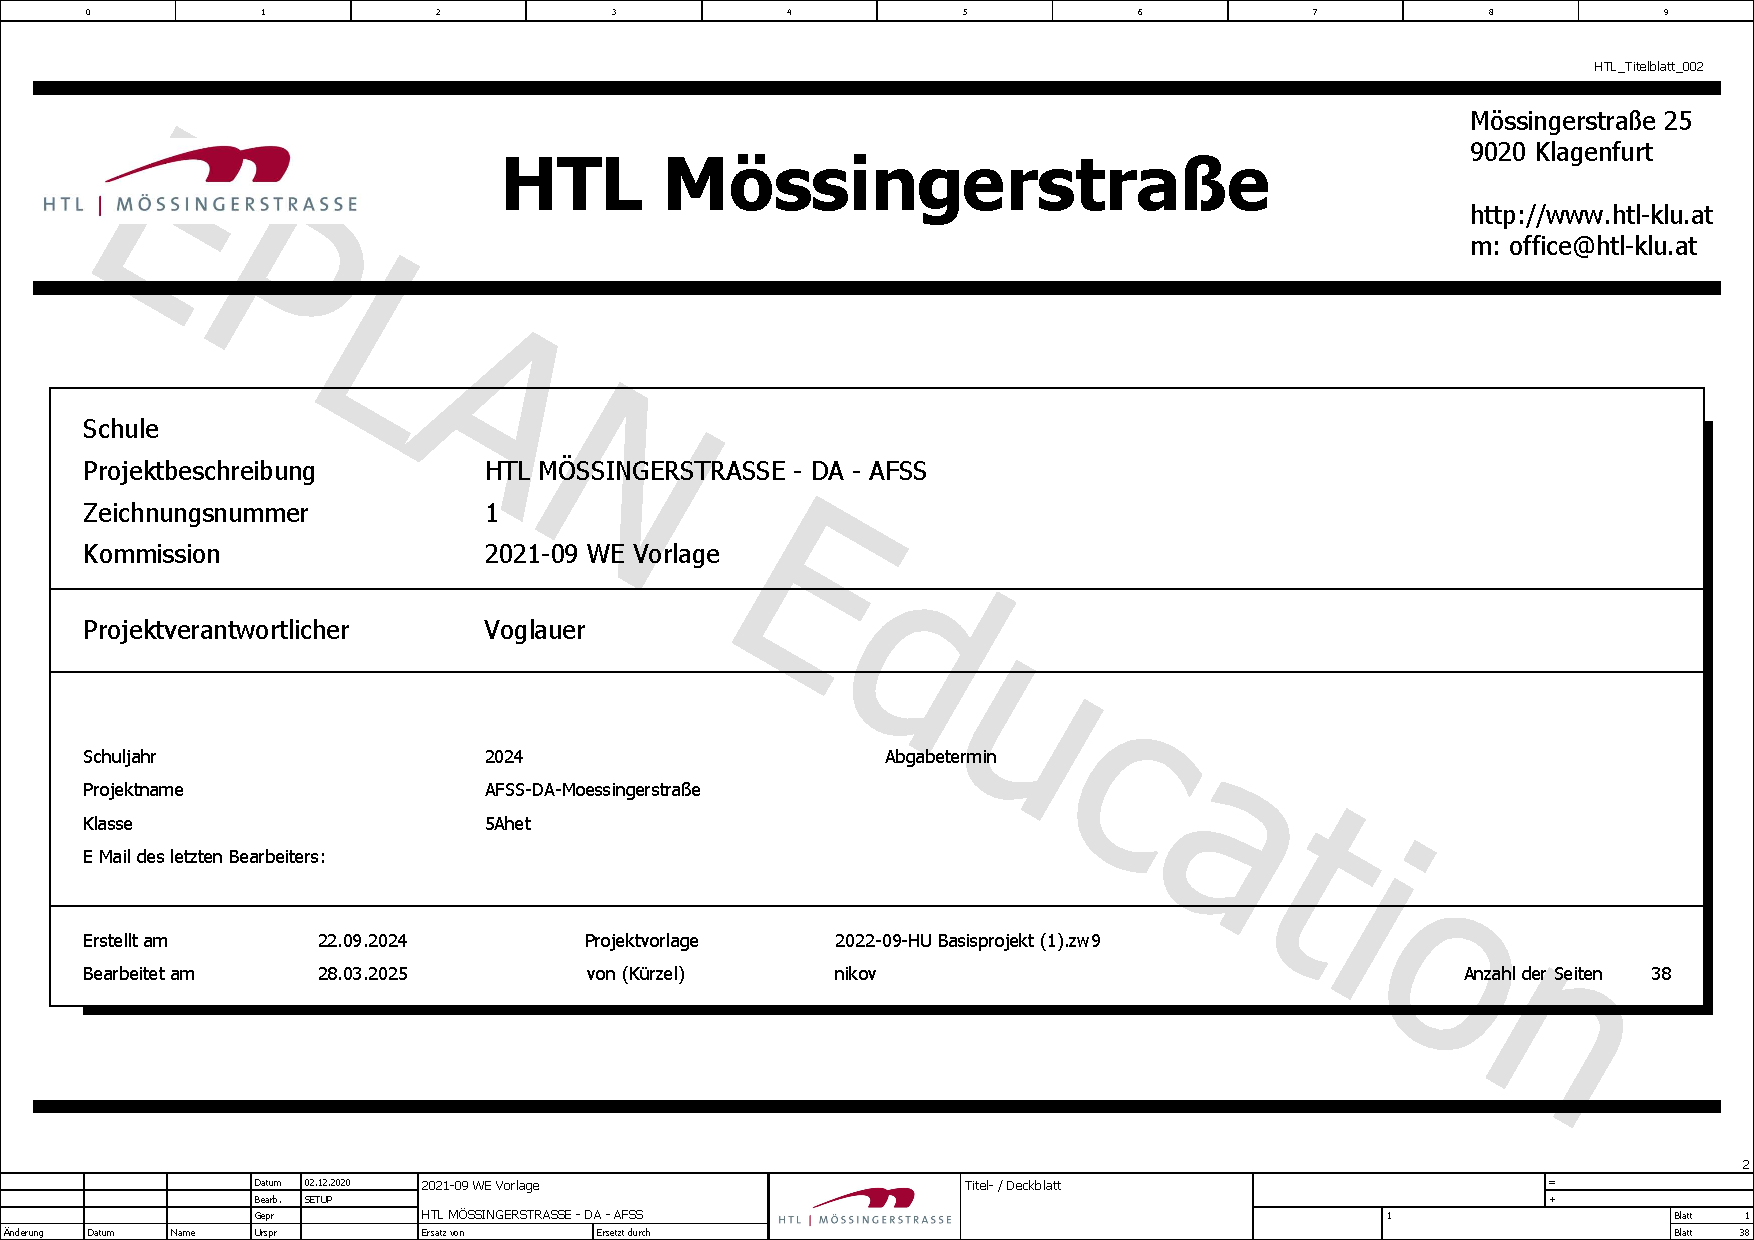
\includepdf[scale = 0.8, offset=-0.25in -0.25in, pages = -, pagecommand={},noautoscale=true, angle=90, flip-other-edge]{Vogis Bilder/Zweiter Druck E-Plan.pdf}


\newpage
\renewcommand{\cftfigpresnum}{Abb. }
\setlength{\cftfignumwidth}{2cm}
\listoffigures

\newpage

\renewcommand{\cfttabpresnum}{Tab. }
\setlength{\cfttabnumwidth}{2cm}
\listoftables
\lstlistoflistings
\end{document}
